\section*{Введение}
\addcontentsline{toc}{section}{Введение}

В настоящей работе рассматривается процесс погружения сваи импульсным погружателем. 
Работа импульсного погружателя основана на действии полигармонического импульса,
создаваемого центробежными силами системы дебалансов, на сваю.

В работе \cite{ermolenko} представлена задача оптимизации устройства погружения свай в грунт. Его характерным отличием стало наличие
нескольких пар дебалансов, которые позволяют создать положительный импульс, действующий на свайный элемент, в несколько раз больший,
чем при классической схеме вибропогружателя \cite{ermolenko_patent}. В дальнейшем данное устройство получило название импульсный погружатель.
Математическая модель работы импульсного погружателя описана в работе \cite{ermolenko_kostin}, а так же поставлена задача оптимизации импульса по
коэффициенту асимметрии. Данная задача оптимизации была решена и описана в работах \cite{kostin_va}, \cite{ermolenko_kostin}.

В то же время, при использовании оптимальных соотношений при проектировании в обязательном порядке закладываются допуски,
которые неизбежны при производстве элементов. Эти несовершенства нарушают форму оптимального импульса. Возникает задача исследования
зависимости импульса от отклонений в параметрах и оценки допустимых значений этих отклонений. Для этого применялась программная реализация
математической модели процесса работы импульсного погружателя, которая легла в основу численного эксперимента.

Таким образом в данной работе ставятся и решаются следующие задачи:
\begin{enumerate}
    \item Описать математическую модель процесса работы импульсного погружателя с дефектами;
    \item Оценить суммарное влияние, вносимое деталями с дефектами и естесвенным износом на процесс погружения;
    \item Оценить влияние на процесс погружения, вносимое каждой деталью в отдельности;
\end{enumerate}

Данная работа состоит из четырёх частей. В первой части описывается математический аппарат вибрационной механики.
Даются основные понятия, а также описываются механические процессы происходящие во время работы погружателя.

Во второй части описывается математическая модель процесса погружения в идеальном случае (без учёта дефектов).
Выводится дифференциальное уравнение второго порядка, которое позволяет рассчитать глубину и время
погружения в зависимости от характеристик устройства, сваи и грунта.
Также приводятся необходимые для дальнейших рассуждения сведения из теории разностных схем.

В третьей части описывается математическая модель процесса погружения с учётом дефектов, связанных с допусками
на производстве и естесвенным износом деталей. Проводится численный эксперимент в котором оценивается влияние
шума на весь процесс погружения.

В четвёртой части ставится и решается задача по определению погрешности, вносимой
каждой из пар дебалансов с дефектами в процесс погружения. Для этого была написана программа,
рассчитывающая коэффициент ассиметрии для различных значений шумов для каждой пары дебалансов.

Целью этой работы является составление математической модели импульсного погружателя с дефектами одной пары дебалансов.
Определение, с использованием полученной модели, номера наиболее значимой пары дебалансов в процессе погружения.
Результатом этой работы будет служить программа, которая решает задачу поставленную выше.

\clearpage

\section{Модель погружателя}

\subsection{Вибрационное погружение и внедрение}

Погружение в грунт тел, подвергаемых действию вибрирования, представляет собой сложное механичекское явление. Вибрационный
погружатель предназначен для погружения (извлечения) свай в песчаные или глинистые грунты. Рассмотрим cхему вибрационного
погружателя (рис. \ref{fig:vp}), а также факторы, играющие наиболее существенную роль в процессе вибрационного погружения.

\begin{figure}[h]
    \centering
    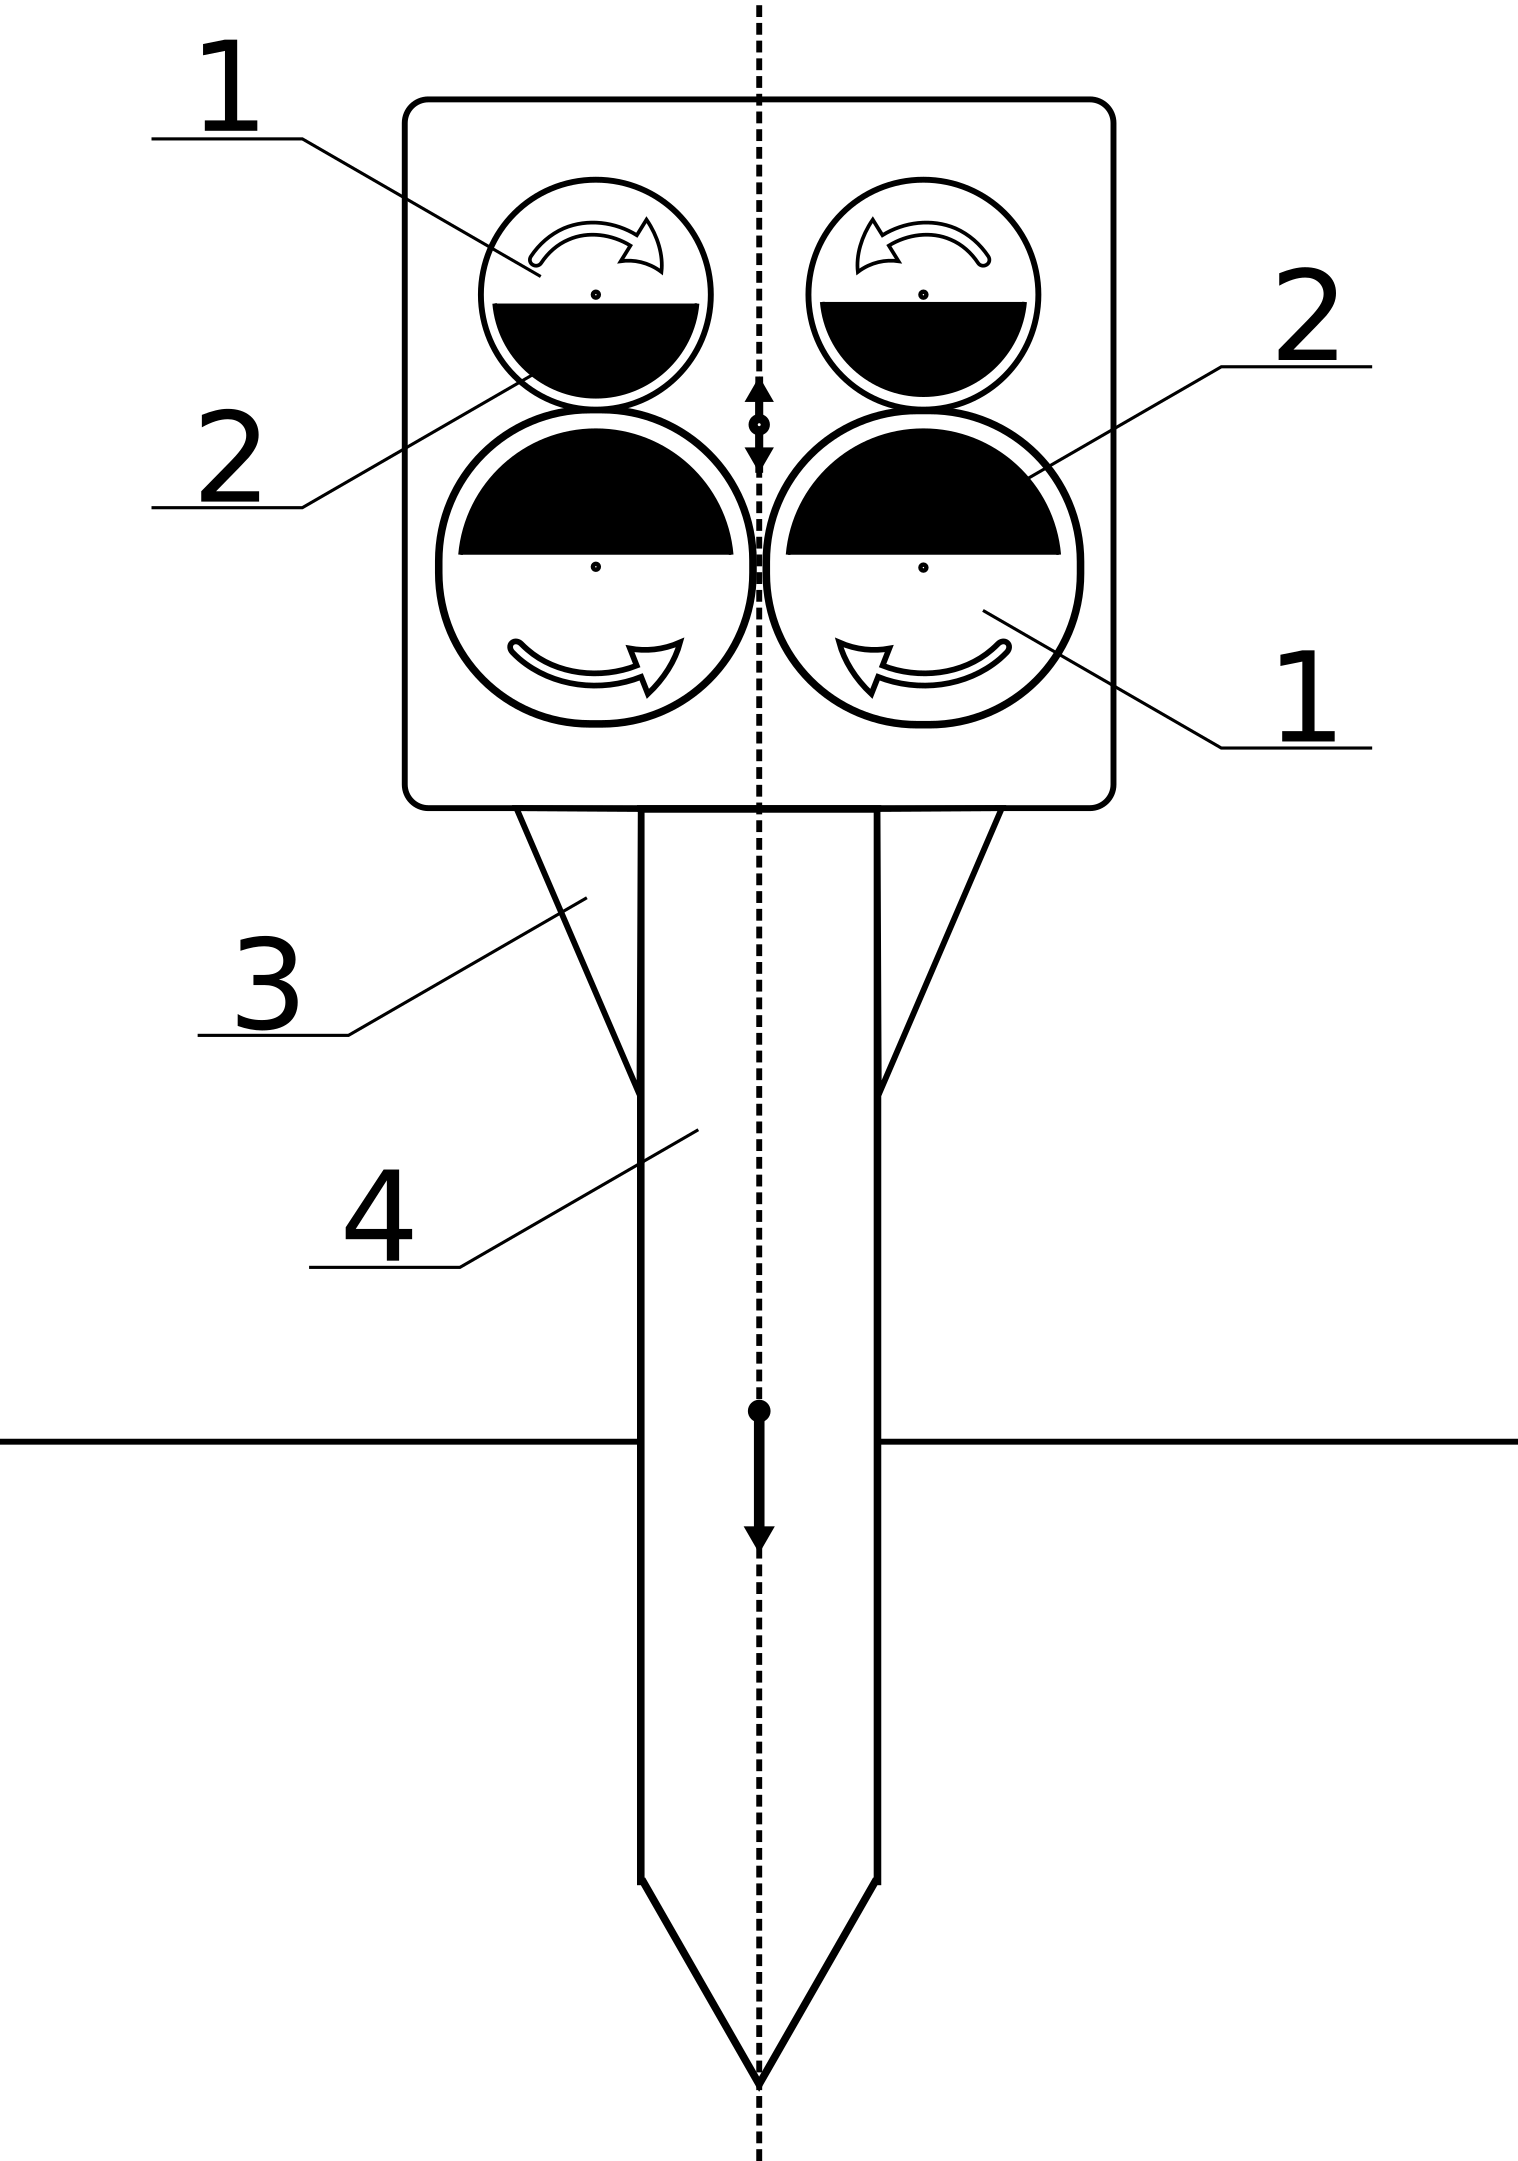
\includegraphics[width=0.4\linewidth]{pogruzhatel-2}
    \caption{Вибрационный погружатель.}
    \label{fig:vp}
\end{figure}

\noindent При вращении \textit{валов} (1) с \textit{дебалансами} (2) на их ось крепления действует центробежная сила
и вибрационный погружатель получает вибрирующее движение, которое сообщается через \textit{наголовник} (3) \textit{свае} (4).

\noindent Вибрационный погружатель генерирует гармоническую силу $\Phi_0 \sin \omega t$,
где $\Phi_0$ - амплитуда колебаний, $\omega$ - частота колебаний и $t$ - время.

\begin{definition}
    Сила, которая меняется с течением времени по гармоническому (синусоидальному или косинусоидальному)
    закону называется гармонической.
\end{definition}

Для выяснения основных закономерностей работы погружателя примем следующее предположение: будем считать, что
при движении сваи вниз сопротивление равно $-F+$, а при движении вверх $F-$, причём $F+ > F-$, т.к. $F-$ обусловлено только
силами сопротивления, распределёнными по боковой поверхности, а $F+$ учитывает также силы сопротивления дейстующие на
торец сваи. \footnote{Более подробно про силы дейстующие на сваю в процессе погружения будет рассказано
в главе (\ref{chapter:newton}).}

Дифференциальное уравнение движения сваи при сделанных предположениях имеет вид:

\begin{equation}
    m\ddot{x} = mg + \Phi_0 \sin \omega t + F(\dot{x}),
\end{equation}
где
\begin{equation}
    \begin{aligned}
        F(\dot{x}) =
        \begin{cases}
            -F_+ \quad \text{при} \quad \dot{x} > 0,\\
            \phantom{-}F_- \quad \text{при} \quad \dot{x} < 0,
        \end{cases}\\
        -F_+ < F(\dot{x}) < F_- \quad \text{при} \quad \dot{x} = 0.
    \end{aligned}
\end{equation}

\begin{definition}
    Вибрационным погружением называют проникновение твёрдого тела в сопротивляющуюся среду
    под действием постоянной и знакопеременной сил.
\end{definition}

\subsection{Математическая модель импульсного погружателя}

Основное отличие импульсного погружателя от вибропогружателя заключается в том, что сила, генерируемая
импульсным погружателем имеет вид гармонических колебаний с явно вырараженными периодическими импульсами и задаётся
по следующему закону:

\begin{equation}
    f(t,\lambda)=\sum_{k=1}^n \lambda_k\cos(kt),\ t\in [-\pi,\pi],\ \lambda =(\lambda_1, \ldots,\lambda_n).
\end{equation}

\noindent На рисунке (\ref{fig:impulse_1vs6}) зелёным представлен график данной функции при $n = 6$ и
$\lambda_1 = \lambda_2 = \ldots = \lambda_6 = 1$.

\begin{figure}[ht]
    \centering
    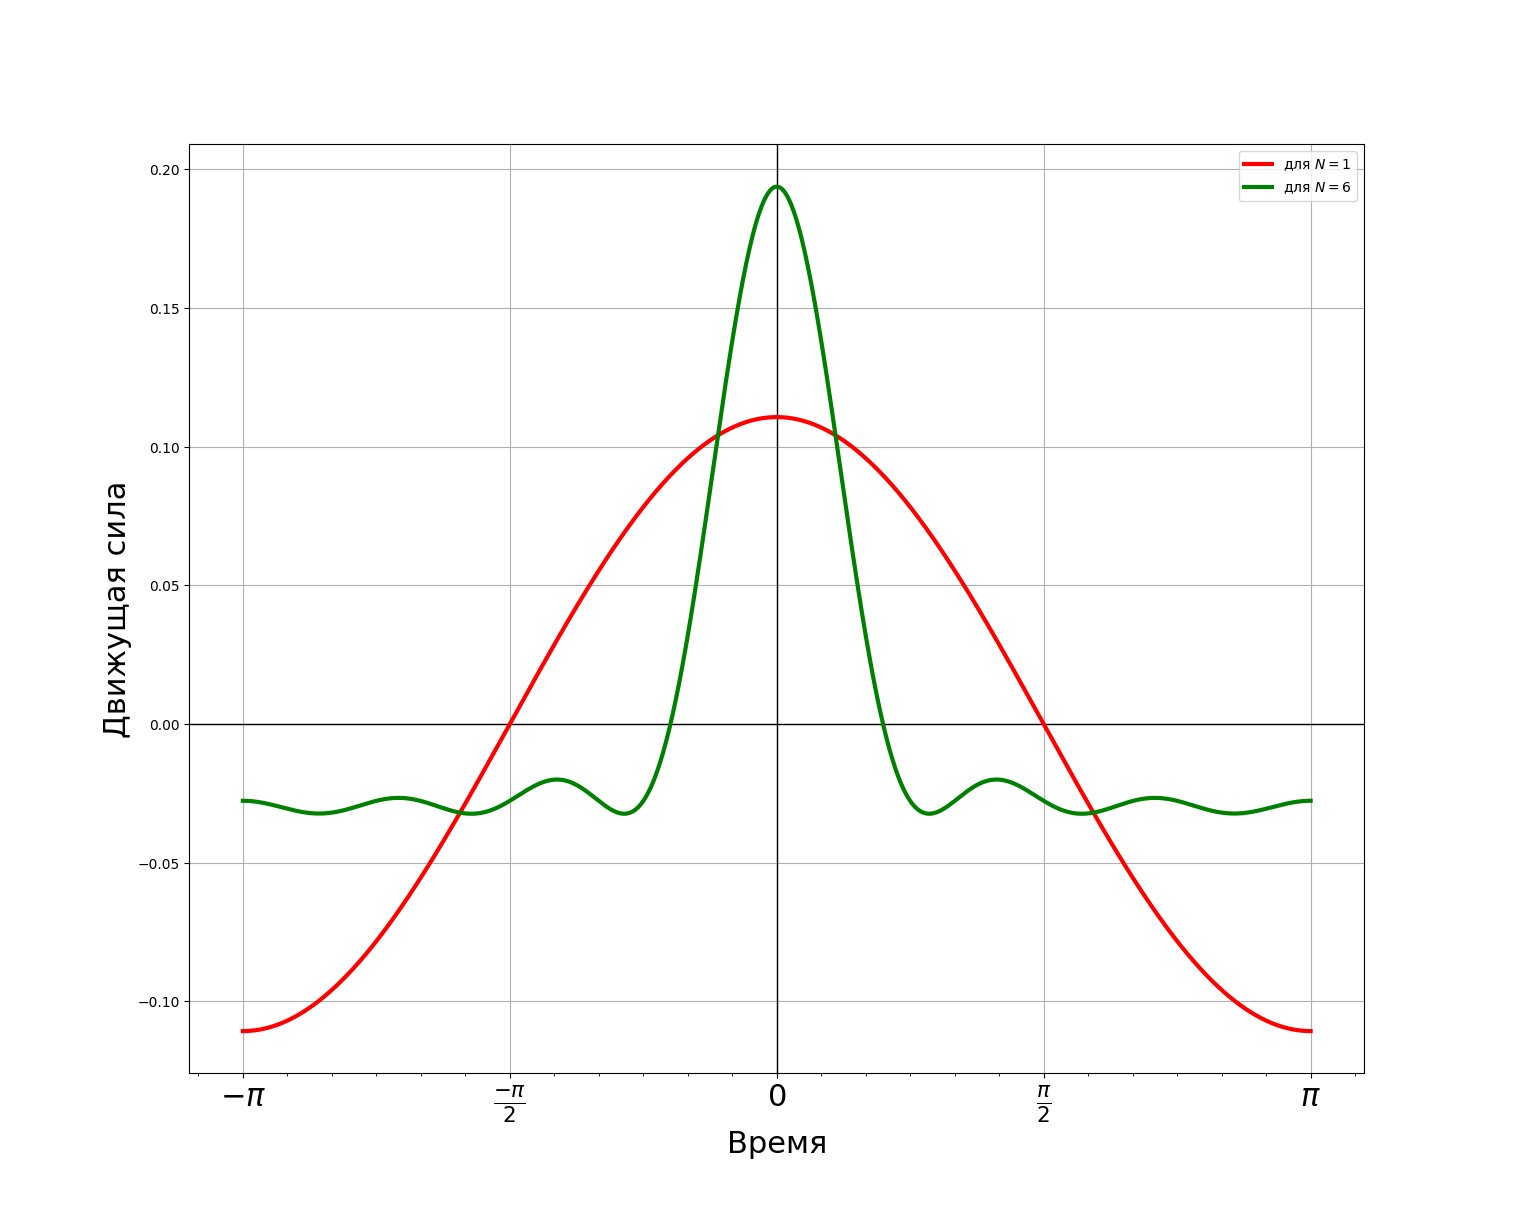
\includegraphics[width=0.8\linewidth]{impulse_1vs6}
    \caption{График функций движущей силы погружателя с одной парой дебалансов (вибрационный погружатель, $N = 1$, красный) и с 6 парами дебалансов (импульсный погружатель, $N = 6$, зеленый) за один период времени.}
    \label{fig:impulse_1vs6}
\end{figure}

\noindent Как видно из данного графика большую часть времени свая стоит на месте т.к. силы, генерируемой погружателем,
недостаточно для преодоления сопротивления грунта. Поэтому, говоря о скорости погружения сваи, будем подразумевать среднюю
скорость погружения.

\begin{definition}
    Под вибрационным внедрением будем понимать внедрение твёрдого тела в сопротивляющуюся среду с заданной
    средней скоростью.
\end{definition}

В работе импульсного погружателя полезной силой считается та, которая направлена на погружение твердого тела в
сопротивляющуюся среду. Для компенсации горизонтальных сил, возникающих при вращении одного дебаланса,
в конструкции погружателя дебалансы используются парами. Их вращение происходит в противоположные стороны, по отношению друг
к другу. В таком случае, уравнение гармонического колебания пары дебалансов будет иметь вид:

\begin{equation}
    \begin{aligned}
        x(t) = 2 m \omega^2 l \cos (\omega t)
    \end{aligned}
\end{equation}
\noindent где $m$ - масса дебаланса, $l$ - расстояние от центра масс до оси вращения дебаланса, $\omega$ - угловая скорость.

\begin{figure}[ht]
    \centering
    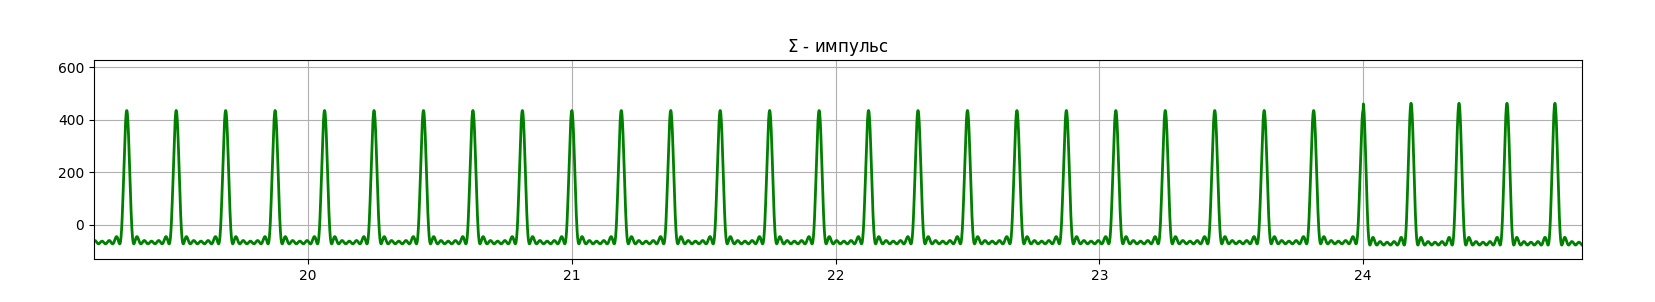
\includegraphics[width=1\linewidth]{graph-impulse}
    \caption{Оптимальный импульс, создаваемый импульсным погружателем.}
    \label{fig:graph-impulse}
\end{figure}

\noindent Для всех пар дебалансов сумма гармонических колебаний будет иметь вид:

\begin{equation}
    \label{eq:F}
    F = \sum\limits_{k = 1}^n 2 m_k \cdot (k \omega)^2 \cdot l(r_k) \cdot \cos (k \omega t)
\end{equation}
\noindent где $n$ --- количество пар дебалансов, $k$ --- порядковый номер пары дебалансов. График данной функции
представлен на рисунке \ref{fig:graph-impulse}.

Абсолютное отношение максимального значения функции к минимальному значению называется коэффициентом асимметрии $K_n$:
\begin{equation}
    \label{eq:asymm-coef}
    K_n = \left| \frac{ \max\limits_{-\pi<t<\pi} F(t)}{\min\limits_{-\pi<t<\pi} F(t)}\right|,
\end{equation}
где $n$ -- число пар дебалансов в импульсном погружателе, $t$ -- время работы в течении одного периода функции $F$.

Этот эффект асимметрии позволил при меньшем весе установки, создавать больший положительный импульс. Таким образом,
критерием оптимизации стал параметр – коэффициент асимметрии. Проблема выбора радиусов дебалансов с наибольшим
коэффициентом асимметрии была решена в работах \cite{kostin_va} и \cite{kostin_dv}, где даётся определение оптимального
импульса и доказывается теорема о выборе параметров оптимального импульсного погружателя.

При построении математической модели погружения сваи будем использовать модель оптимального импульсного погружателя,
заданную с точностью до констант формулой:

\begin{equation}
    \label{eq:impulse_mf}
    f_n(t, \lambda) = \sum\limits_{k = 1}^n (n-k+1) \cos(k \omega t),\ t \in [-\pi, \pi],\ \lambda =(\lambda_1, \ldots,\lambda_n)
\end{equation}

\noindent где $\omega$ -- скорость вращения первой пары дебалансов. Функция (\ref{eq:impulse_mf}) называется импульсом Максвелла–Фейера.
Период $t \in [-\pi, \pi]$ соответствует полному обороту наибольшего по радиусу дебаланса. Данный отрезок выбран для удобства
математического формализации задачи. На практике и численном эксперименте длина периода зависит от скорости вращения $\omega$, которая
изменяется при управлении работой погружателя.

~\

\noindent Основные параметры вибрационного внедрения:
\begin{enumerate}
    \item Глубина погружения;
    \item Скорость погружения.
\end{enumerate}
На данный процесс оказывают влияние следующие параметры системы:
\begin{enumerate}
    \item Длина сваи;
    \item Форма и площадь сечения сваи;
    \item Тип грунта.
\end{enumerate}

\subsection{Описание процесса вибропогружения в терминах ньютоновской механики}
\label{chapter:newton}

Расммотрим более подробно силы, действующие на сваю в процессе погружения. Примем несколько допущений:

\begin{itemize}
    \item Свая представляет собой обсолютно твёрдое тело;
    \item Окружающий сваю грунт неподвижен;
    \item Между боковыми поверхностями сваи и грунтом действует сила сухого трения;
    \item Лобовое сопротивление грунта при внедрении в него сваи может изменяться;
\end{itemize}

\noindent Дадим следующие определения:

\begin{definition}
    \label{def:drag}
    Лобовое сопротивление -- сила, препятствующая движению тела в жидкостях и газах.
\end{definition}

\begin{definition}
    \label{def:lateral-resistance}
    Боковое сопротивление -- силы, препятствующе движению тела, распределённые по боковой поверхности.
\end{definition}

\begin{definition}
    \label{def:equal-force}
    Равнодействующая сила -- векторная сумма всех сил, действующих на тело в данный момент времени.
\end{definition}

С учётом этих данных процесс вибрационного погружения можно описать с помощью нескольких этапов.

~\

\noindent\textit{Сила вибрационного воздействия направлена вверх:}

\begin{equation*}
    R = - F_\text{вибр. возд.} + F_\text{тяж.} + F_\text{бс},
\end{equation*}
где
\begin{equation*}
    \begin{aligned}
        &R - \text{равнодействующая сила,}\\
        &F_\text{вибр. возд.} - \text{сила, создаваемая погружающей установкой,}\\
        &F_\text{тяж.} - \text{сила тяжести,}\\
        &F_\text{бс} - \text{сила бокового сопротивления.}
    \end{aligned}
\end{equation*}

\noindent На данном этапе погружающая установка тянет сваю вверх, преодолевая силу тяжести
и сопротивление грунта по боковой поверхности. Стоит заметить, что в случае с импульсным погружателем, сила тяжести и
сила бокового сопротивления уравновешивают силу вибрационного воздействия, направленную вверх. Таким образом свая, которая
хорошо переносит сильное сжатие, но разрушается при попытке растяжения остаётся целой.

~\

\noindent\textit{Сила вибрационного воздействия направлена вниз:}

\begin{equation}
    \label{eq:R}
    R = F_\text{вибр. возд.} + F_\text{тяж.} - F_\text{бс} - F_\text{лс},
\end{equation}
где
\begin{equation*}
    F_\text{лс} - \text{сила лобового сопротивления (\ref{def:drag})}
\end{equation*}

\noindent На текущем этапе появляется сила сопротивления грунта на торце сваи. Если сила погружающей установки и сила тяжести
не смогут превысить сопротивление грунта, то погружение остановится. После этого этапа происходит остановка системы, до тех
пор, пока вынуждающей силы не станет достаточно чтобы поднять сваю вверх ($F_\text{вибр. возд.} > F_\text{тяж.} + F_\text{бс}$),
после чего цикл повторяется.

В дальнейшем будем пользоваться уравнением (\ref{eq:R}) для численного моделирование процесса, т.к. оно содержит все силы
действующие на систему в разные моменты времени.

\clearpage

\section{Численное моделирование}

Распишем равенство (\ref{eq:R}) более подробно. Через $m$ обозначим массу всей установки, через $x(t)$ - глубину
погружения сваи, а через $t$ - время погружения сваи. Получаем:

\begin{itemize}
\item Согласно второму закону Ньютона $R = ma = m\ddot{x}$, где $m$ - масса и $a$ - ускорение.
\item $F_\text{тяж.} = mg$, где $g$ - ускорение свободного падения.
\item $F_\text{лс} = S_\text{пс} h_i(x(t), \xi)$, где $S_\text{пс}$ - площадь поперечного сечения сваи,
$h_i(x(t), \xi)$ - удельное лобовое сопротивление, $\xi$ - коэфициент условий работы грунта под нижним концом сваи.
\item $F_\text{бс} = P x(t) f_i(\psi)$ - сила бокового сопротивления, представляющая собой произведение периметра сваи
$P$, глубины погружения $x(t)$ и удельной силы бокового сопротивления $f_i(\psi)$, зависящей от типа грунта.
\end{itemize}

\noindent Будем считать, что в момент времени $t = 0$ свая ещё не начала погружаться т.е. глубина погружения равна 0.
Исходя из этого получаем следующее дифференциальное уравнение второго порядка:

\begin{equation}
    \label{eq:main}
    m\ddot{x} = F_\text{вибр. возд.} + mg + S_\text{пс} h_i(x(t), \xi) + P x(t) f_i(\psi)
\end{equation}
с начальными условиями:
\begin{equation}
    \label{eq:main-conditions}
    x(0) = \dot{x}(0) = 0
\end{equation}

Решение данного уравнения позволяет определить время и глубину погружения в зависимости от характеристик погружающей
установки, размеров и веса сваи, а также типа грунта.

\subsection{Необходимые сведения из теории разностных схем}

Для того, чтобы описать дифференциальное уравнение, используя разностную схему необходимо сделать следующее:
\begin{enumerate}
    \item Заменить область непрерывного изменения аргумента областью дискретного изменения;
    \item Заменить дифференциальный оператор некоторым разностным оператором;
    \item Заменить начальные и краевые условия их разностным аналогом.
\end{enumerate}

При решении задач с использованием разностного метода мы не можем написать разностные решения для всех возможных аргументов,
поэтому мы выберем несколько точек и будем приближённо искать решение только в этих точках. Такую совокупность точек
называют сеткой (\ref{eq:grid}).

\begin{definition}
    \label{eq:grid}
    Сетка - множество точек, заданных в области определения некоторой функции.
\end{definition}

Теперь дадим определение разностной аппроксимации.

\begin{definition}
    Пусть дан дифференциальный оператор $L$, действующий на функцию $f = f(x)$. Если заменить все входящие в $L(f)$
    производные разностными отношениями, то мы получим разностное выражение $L_h(f_h)$. Такая приближённая замена называется
    аппроксимацией дифференциального уравнения разностным оператором.
\end{definition}

Существует множество разностных выражений, аппроксимирующих $L(f)$. Например, пусть $L(f) = \frac{df}{dx}$. Тогда для его
аппроксимации можно воспользоваться любым из следующих выражений:

\begin{equation}
    \label{eq:lx-plus}
    L_h^+f = \frac{f(x + h) - f(x)}{h}
\end{equation}

\begin{equation}
    \label{eq:lx-minus}
    L_h^-f = \frac{f(x) - f(x - h)}{h}
\end{equation}

\begin{equation}
    \label{eq:lx-center}
    L_h^0f = \frac{f(x + h) - f(x - h)}{2h}, \text{ где } h = 0,5
\end{equation}

\noindent Здесь $h$ - шаг сетки. Выражение (\ref{eq:lx-plus}) называется правая разностная производная, (\ref{eq:lx-minus})
- левая разностная производная и (\ref{eq:lx-center}) - центральная разностная производная.

\subsection{Разностная схема}

Будем решать дифференциальную задачу (\ref{eq:main}) приближённо, с использованием разностной схемы. Для этого дадим следующее
определение:

\begin{definition}
    Совокупность разностных уравнений, апроксимирующих основное дифференциальное уравнение, и дополнительные
    (краевые и начальные) условия называется разностной схемой.
\end{definition}

Рассмотрим разностную аппроксимацию дифференциальных операторов $L_x = \dot{x}$ и $L_{xx} = \ddot{x}$ на равномерной сетке
с шагом $h$:

\begin{equation}
    L_x = \frac{dx}{dt} = \frac{x(t + h) - x(t)}{h}
\end{equation}
\begin{equation}
    \label{eq:lxx}
    L_{xx} = \frac{d^2x}{dt^2} = \frac{\dot{x}(t + h) - \dot{x}(t)}{h} = \frac{x(t + h) - 2x(t) + x(t - h)}{h^2}
\end{equation}
Перепишем равенство (\ref{eq:lxx}) в виде:
\begin{equation}
    \label{eq:approximation}
    \frac{x_{i+1} - 2x_i + x_{i-1}}{h^2},
\end{equation}
где $x_i = x(t_i), t_{i+1} = t_i + h$.

~\

\noindent Заменим $\ddot{x}$ в уравнении (\ref{eq:main})-(\ref{eq:main-conditions}) разностной аппроксимацией (\ref{eq:approximation}):
\begin{equation}
    \label{eq:result}
    \begin{aligned}
        m\frac{x_{i+1} - 2x_i + x_{i-1}}{h^2} = F_\text{вибр. возд.} + mg + S_\text{пс} h_i(x(t), \xi)+ P x(t) f_i(\psi)\\
        x_{i+1} - 2x_i + x_{i-1} = \frac{h^2}{m}(F_\text{вибр. возд.} + mg + S_\text{пс} h_i(x(t), \xi) + P x(t) f_i(\psi))\\
        x_{i+1} = 2x_i - x_{i-1} + \frac{h^2}{m}(F_\text{вибр. возд.} + mg + S_\text{пс} h_i(x(t), \xi) + P x(t) f_i(\psi))
    \end{aligned}
\end{equation}

\noindent Получили рекуррентное равенство, которое позволяет расчитать текущее значение $x$, зная два предыдущих значения. Будем
считать, что $x_0 = x_1 = 0$.

\clearpage

\section{Моделирование допусков на изготовление и различных дефектов устройства}

Предложенный теоретический импульс, создаваемый импульсным погружателем, имеет наивысший
коэффициент асимметрии равный числу пар дебалансов $K_n=n$ \cite{kostin_va}. При этом важно подчеркнуть, что
чем больше число звеньев и выше скорость оборотов, тем краткосрочнее действие импульса. Этот факт заставляет
внимательнее изучать вопрос устойчивости и достижения оптимальной амплитуды. Ведь если скорость вращения валов
увеличится до значений, при которых пик импульса будет как бы «срезаться», то значение коэффициента асимметрии
перестанет быть оптимальным, а значит основной принцип импульсного погружателя будет нарушен, процесс погружения
замедлится или вообще остановится, не достигнув теоретически возможных значений.

Отличия практической реализации от теоретического расчета вызваны двумя источниками, первый это не идеальность изготовления,
а второй это уникальные свойства грунта. В настоящей работе проводится исследование устойчивости модели к первому типу
источника погрешности: дефектов конструкции. Вводится дополнительный параметр погрешности в слагаемое вынуждающей силы
$F_{\text{вибр. возд.}}$. При этом погрешность будет как постоянной, вызванной допусками на изготовление, так и случайной,
в следствии несовершенства электродвигателя и ременной передачи.

В качестве основных дефектов можно выделить:
\begin{itemize}
    \item дефекты ременных передач;
    \item дефекты подшипников;
    \item дефекты шкивов;
\end{itemize}
Например, при дефекте шкивов появляется перекос и несоосность с валом, что приводит к периодическому изменению натяжения ремня.
Это же, в свою очередь выражается в модуляции низкочастотной вибрации передачи и сил трения в подшипниках с частотой вращения дефектного шкива.
Непараллельность валов приводит к возникновению периодических ударных нагрузок на ремень с частотой вращения одного из шкивов (или обоих),
импульсно модулирующих силы трения в подшипниках передачи и высокочастотную вибрацию этих подшипников.

В настоящей работе рассмотрен случай, когда скорость вращения валов, соединенных ременной передачей, происходит в поле белого шума.
Эта постановка задачи приходит из практической реализации деталей конструкций и всевозможных дефектов элементов погружающей установки.
Важно отметить, что полученные теоретически результаты для получения оптимального импульса зависят от отношения угловых скоростей дебалансов
и при их даже незначительной рассинхронизации может привести значительному отклонения оптимального значения и изменению важного параметра
процесса погружения – скорости.

Все вышеперечисленное является также дополнительным условием на соотношение частот вращения валов дебалансов,
что приводит к следующей модели:
\begin{equation}
    \widetilde{\omega} = \omega (1 + \delta(t)),
\end{equation}
где $\delta(t)$ - погрешность угловой скорости вращения вала дисбаланса в момент времени $t$, вызванная описанными выше дефектами узлов погружателя.

Т.о. выражение (\ref{eq:F}) примет вид:

\begin{equation}
    \label{eq:F_noise}
    \begin{gathered}
        F = \sum\limits_{k = 1}^n 2 m_k \cdot (k \omega (1 + \delta(t)))^2 \cdot l(r_k) \cdot \cos (k \omega (1 + \delta(t)) t)
    \end{gathered}
\end{equation}

Для выбора модели такой погрешности в настоящей работе предлагается модель белого шума или аддитивного
гауссовского распределения -- обобщенный стационарный случайный процесс $X(t)$ с постоянной спектральной
плотностью и нормальным законом распределения стандартного отклонения \cite{yakovleva}.

\begin{definition}
    Аддитивный шум -- это вид шума, который суммируется с полезным сигналом и статистически не зависим
    от сигнала.
\end{definition}

В численном эксперименте будем рассматривать различные порядки стандартных отклонений случайной
величины $\sigma(\delta)$, описывающей шум в ременной передаче, и оценивать насколько это влияет на
основные характеристики процесса погружения.

\subsection{Численный эксперимент}

Для проведения численного эксперимента были выбраны следующие условия. Импульсный погружатель имеет 6 пар дебалансов $N=6$,
радиусы которых подобраны таким образом, что импульс вынуждающей силы является оптимальным и его коэффициент асимметрии равен $K=6$.
Из инженерных таблиц для грунта типа песок были выбраны $h_i(x(t),x_i)$, – удельное лобовое сопротивление, $\xi$ – коэффициент
условий работы грунта под нижним концом сваи, а также $f_i(\psi)$ – удельной силы бокового сопротивления.

Условие останова при расчете осуществлялся при выполнение любого из условий:
\begin{itemize}
    \item Погружение сваи на глубину $x(t)$ = 4 м. -- свая погружена;
    \item Превышение максимального значения числа оборотов первой пары дебалансов $\max(\omega)$ = 3000 об / мин.
    и при этом свая не погружена.
    \item Отрицательная вынуждающая сила превысит сумму силы тяжести и силы бокового сопротивления $F_\text{вс} > F_\text{бс} + mg $,
    т.к. это может привести к разрушению бетонных свай, которые хрупки к деформации растяжения.
\end{itemize}
В качестве стандартного отклонения были взяты четыре величины: $\sigma(\delta) = 10^{-2}, 10^{-3}, 10^{-4}$, а так же идеальный случай.

\begin{figure}[ht]
    \centering
    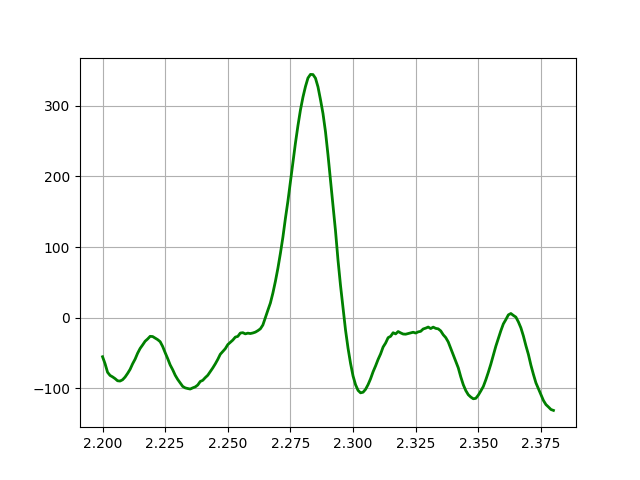
\includegraphics[width=0.45\linewidth]{noise_001}
    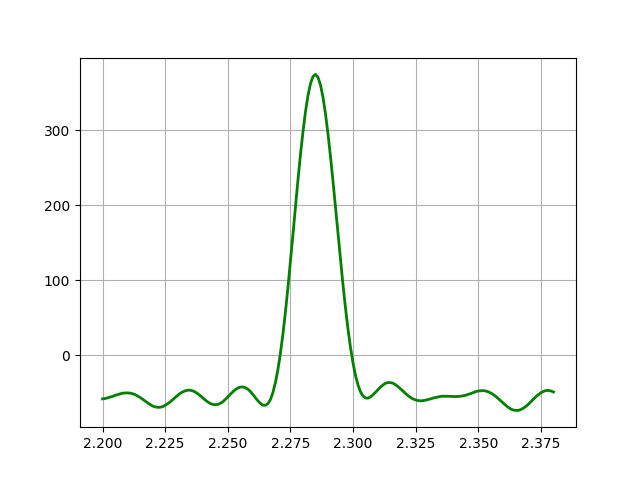
\includegraphics[width=0.45\linewidth]{noise_0001}

    a. $\sigma = 10^{-2}$ \hspace{5cm} b. $\sigma = 10^{-3}$

    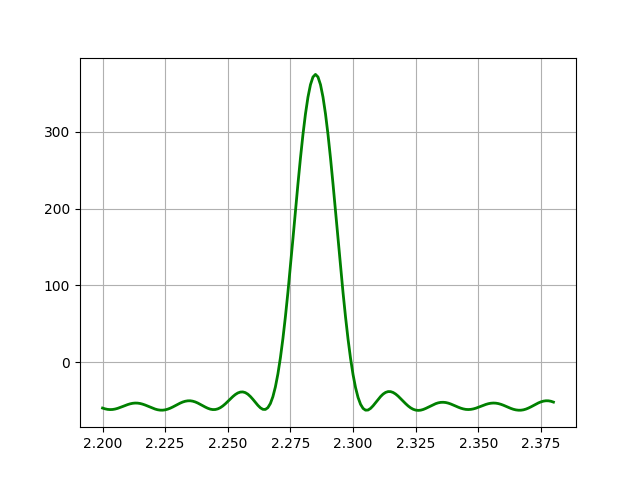
\includegraphics[width=0.45\linewidth]{noise_00001}
    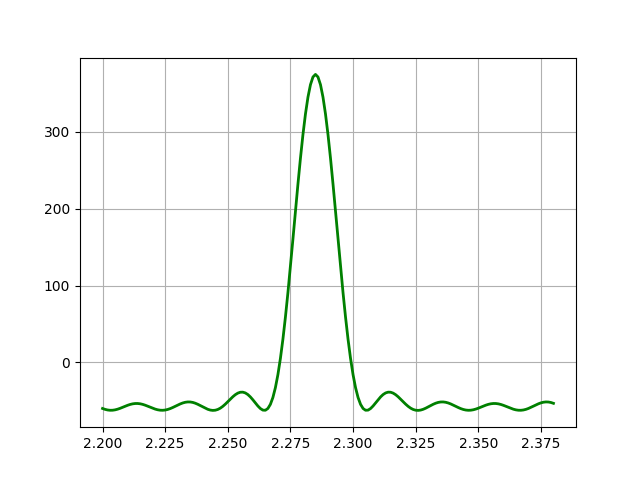
\includegraphics[width=0.45\linewidth]{noise_0}

    c. $\sigma = 10^{-4}$ \hspace{5cm} d. $\sigma = 0$
    \caption{График импульса вынуждающей силы.
    $a$ -- в поле шума со стандартным отклонением $\sigma = 10^{-2}$;
    $b$ -- в поле шума со стандартным отклонением $\sigma = 10^{-3}$;
    $c$ -- в поле шума со стандартным отклонением $\sigma = 10^{-4}$;
    $d$ -- идеальный случай, без шума.}
    \label{fig:impulse-noise}
\end{figure}

При $\sigma > 10^{-3}$ вычисление заканчивается выполнением второго условия, т.е. свая не была погружена на требуемую глубину.
Это означает, что рассинхронизация вращения дебалансов приводит не только к значительному уменьшению коэффициента асимметрии,
но и к неустойчивому поведению погружателя. Такие большие значения шума быстро диагностируются в ходе работы и их стараются не
допускать, проводя устранение дефектов.

С практической точки зрения наиболее интересен результат при $\sigma(\delta) \leq 10^{-3}$. Так как при таком шуме, диагностировать
неисправность затруднительно. Результат моделирования показал, что при $\sigma(\delta) = 10^{-3}$ свая погружается, но не до конца,
то есть вычисления заканчиваются при выполнение второго (достигается максимальная частота работы погружателя). Графическое представление
это случая приводится на рисунке \ref{fig:dive_with_noise}.

\begin{figure}[ht]
    \centering
    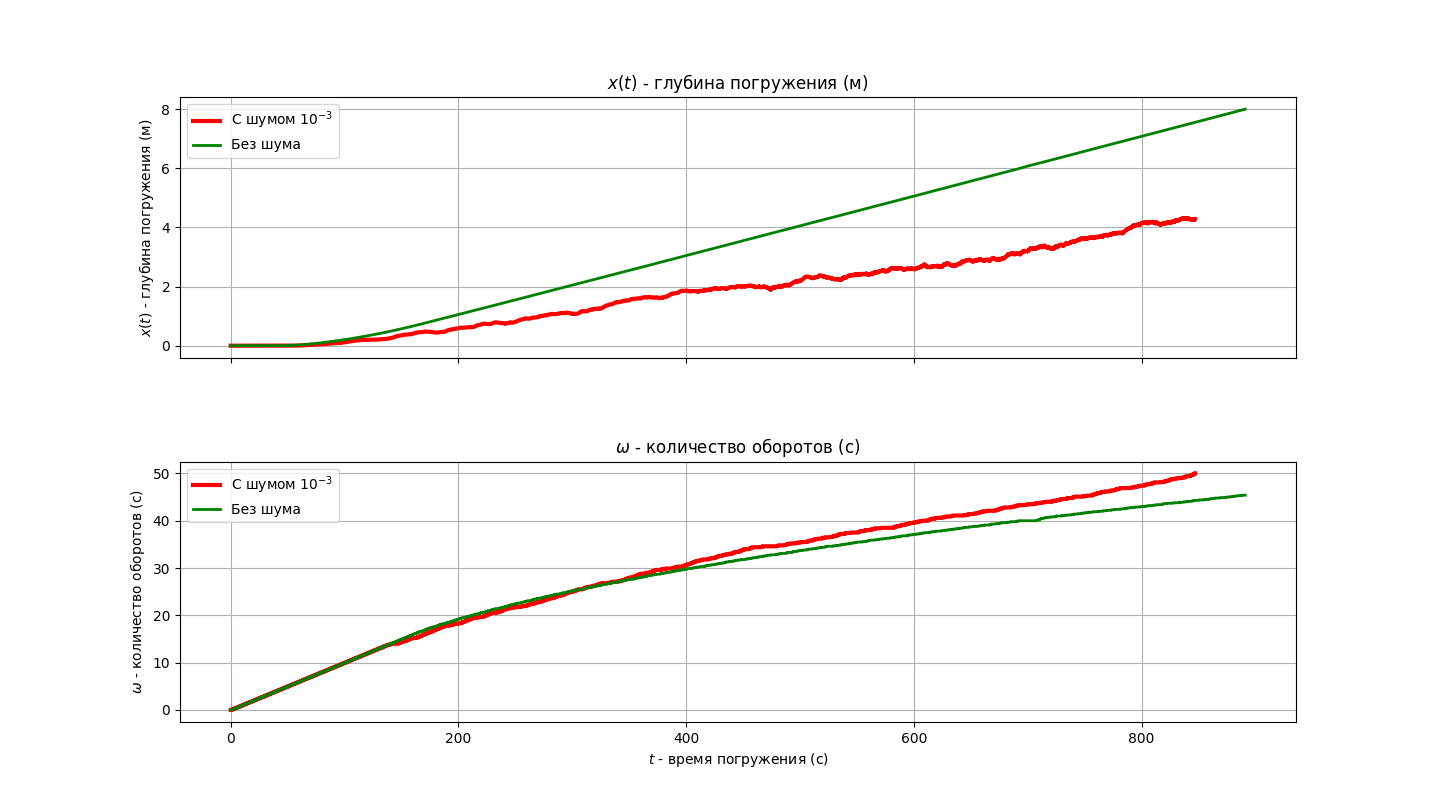
\includegraphics[width=1\linewidth]{dive_with_noise}
    \caption{Графики угловых скоростей и глубины погружения сваи в грунт.
    Зеленый -- идеальный случай; красный -- поле шума со стандартным отклонением $\sigma = 10^{-3}$}
    \label{fig:dive_with_noise}
\end{figure}

Погружение сваи на требуемую глубину (условие останова 1) происходит лишь в отсутствии поля шума или
при стандартном отклонении $\sigma \leq 10^{-4}$. Импульс при этом незначительно изменяет коэффициент асимметрии,
что показывает и визуальное сравнение графиков c и d на рисунке \ref{fig:impulse-noise}.

Исходя из вышесказанного можно сделать вывод об адекватности построенной математической модели. Результаты численного
эксперимента показали, что при большом стандартном отклонении поля белого шума $\sigma(\delta) \geq 10^{-3}$ работа
импульсного погружателя невозможна или крайне затруднительна. С другой стороны, при изготовлении агрегатов обязательно
присутствуют допуски и погрешности, а также в ходе эксплуатации появляются различные дефекты. Но если их суммарное отклонение
будет в допустимых пределах, то предложенная оптимальная конструкция импульсного погружателя будет к ним устойчива.

\section{Влияние на коэффициент асимметрии каждой пары дебалансов с дефектами}

В предыдущем разделе мы задавали случайное изменение угловой скорости вращение дебалансов и смотрели, как меняется характер погружения.
Следующим шагом выясним влияние погрешности изготовления для каждой пары дебалансов в отдельности. Т.е. определим для какой пары шум вносит
наибольшее снижение коэффициента асимметрии и, следовательно, времени погружения.

Вынуждающая сила импульсного погружателя, при наличии отклонения в угловой скорости $m$-го дебаланса:
\begin{equation}
    \label{eq:F_noise_one_deb}
    \widetilde{F} = \sum\limits_{k = 1}^n (n - k + 1) \cdot \cos (k \omega (1 + \delta_k) t),
\end{equation}
где
\begin{equation}
    \begin{aligned}
        \delta_k =
        \begin{cases}
            0, \quad k \neq m \\
            \varepsilon, \quad k = m,
        \end{cases}
    \end{aligned}
\end{equation}

На рисунке \ref{fig:pairs_with_defects_7}, показаны значения коэффициента асимметрии для каждой
пары дебалансов (ось ординат) и погрешности изготовления (ось абсцисс).

\begin{figure}[ht]
    \centering
    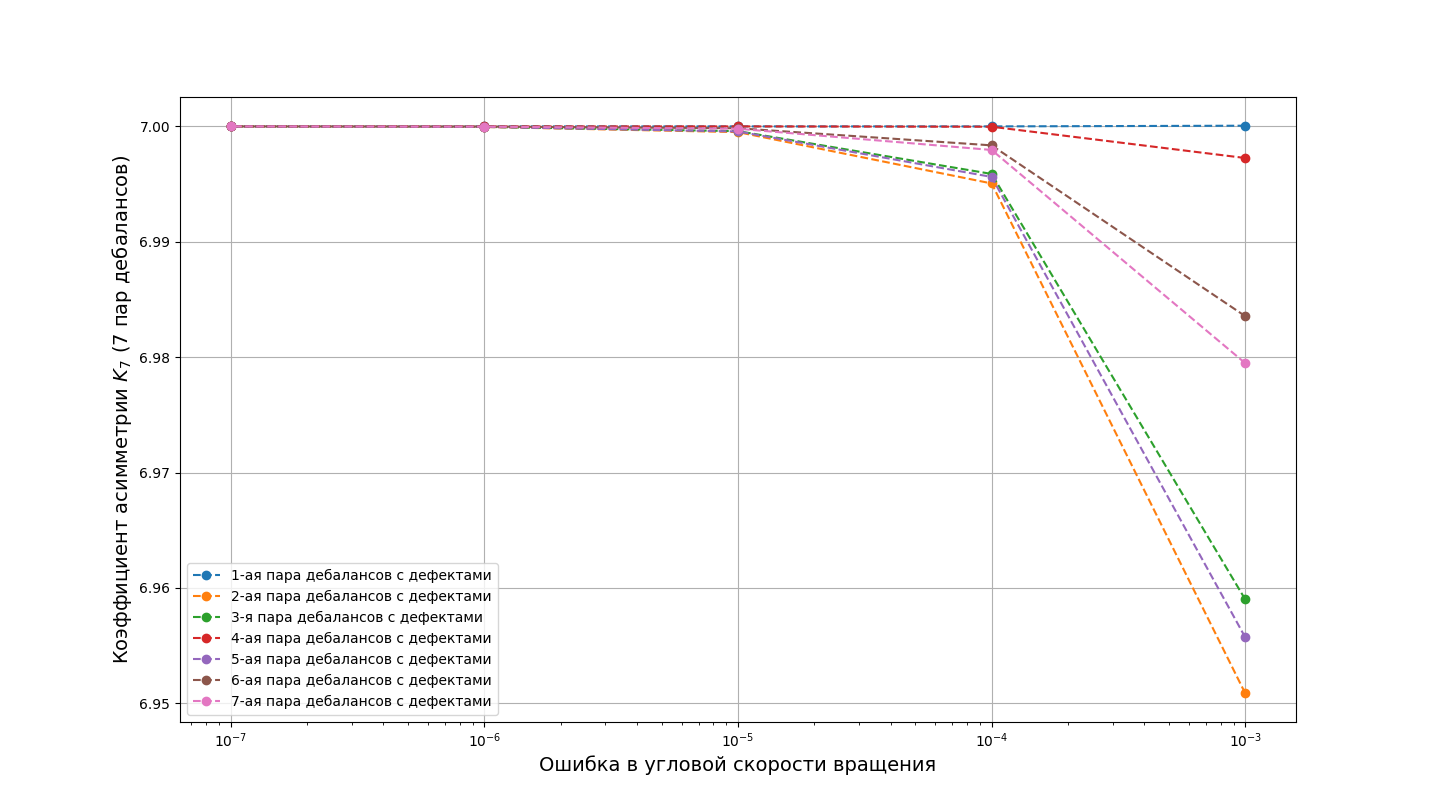
\includegraphics[width=1\linewidth]{pairs_with_defects_7}
    \caption{График изменения коэффициента ассиметрии для каждой пары дебалансов и погрешностей изготовления.
    Количество пар дебалансов -- 7.}
    \label{fig:pairs_with_defects_7}
\end{figure}

В ходе численных расчетов было установлено, что погрешности первой (наибольшей) пары дебалансов приводят к наибольшему отклонению коэффициента
асимметрии и тем самым к снижению эффективности импульсного подводного устройства. Этот результат расширяет и уточняет результат из предыдущего раздела.
Поскольку допуски на изготовление теперь можно определить для каждого звена импульсного погружателя.

Интерсно, что в случае четного числа пар дебалансов и при достижении погрешности изготовления на наименьшей паре свыше $10^{-3}$ наблюдается рост
коэффициента асимметрии (рис. \ref{fig:pairs_with_defects_even}) Этот факт можно трактовать как переход в следующее состояние,
когда число пар дебалансов на одну больше, а значит, коэффициент асимметрии больше. В то же время, при нечетном числе пар дебалансов
наблюдается традиционная закономерность простого уменьшения коэффициента асимметрии.
Изучение этого факта требует более тщательного исследования.

\begin{figure}[ht]
    \centering
    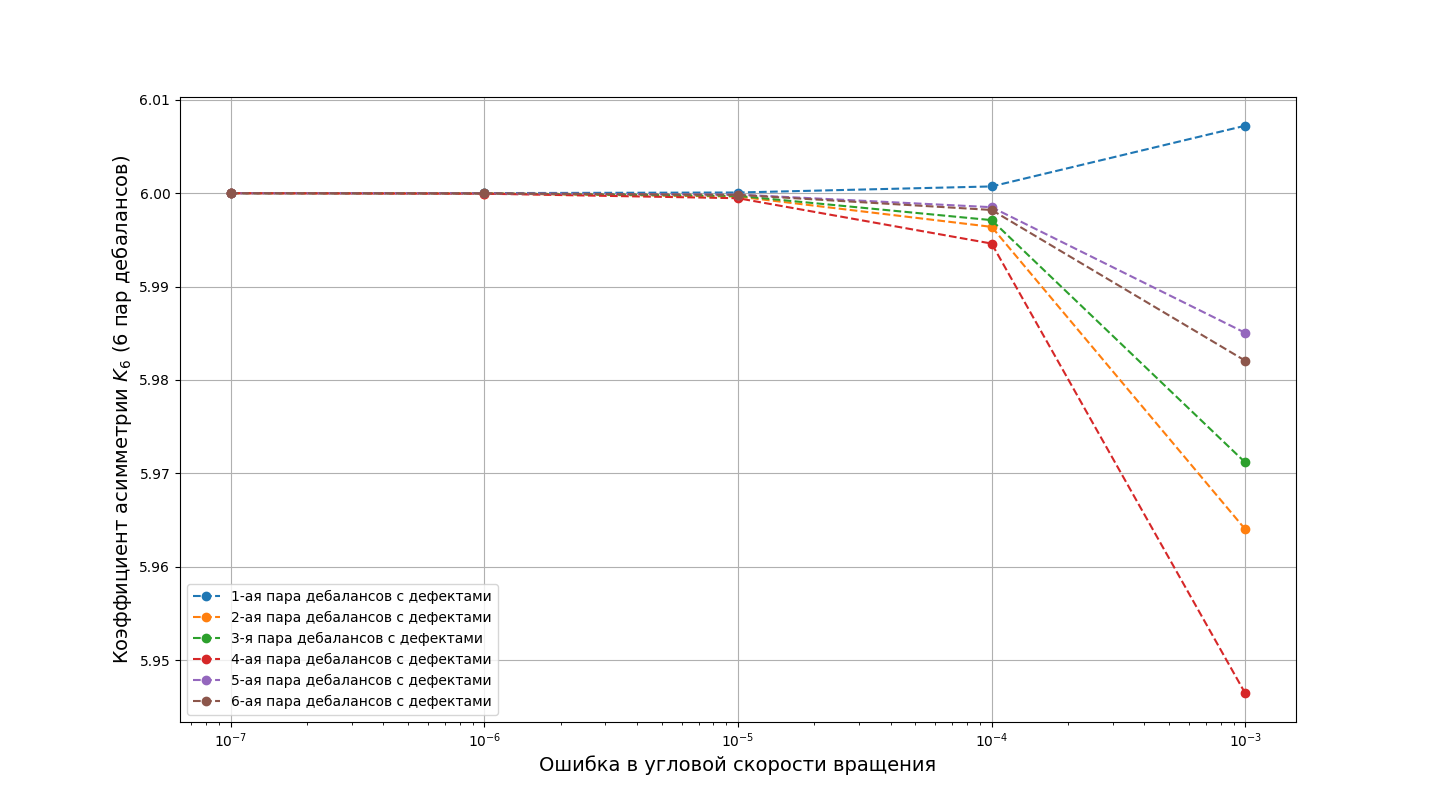
\includegraphics[width=1\linewidth]{pairs_with_defects_6}
    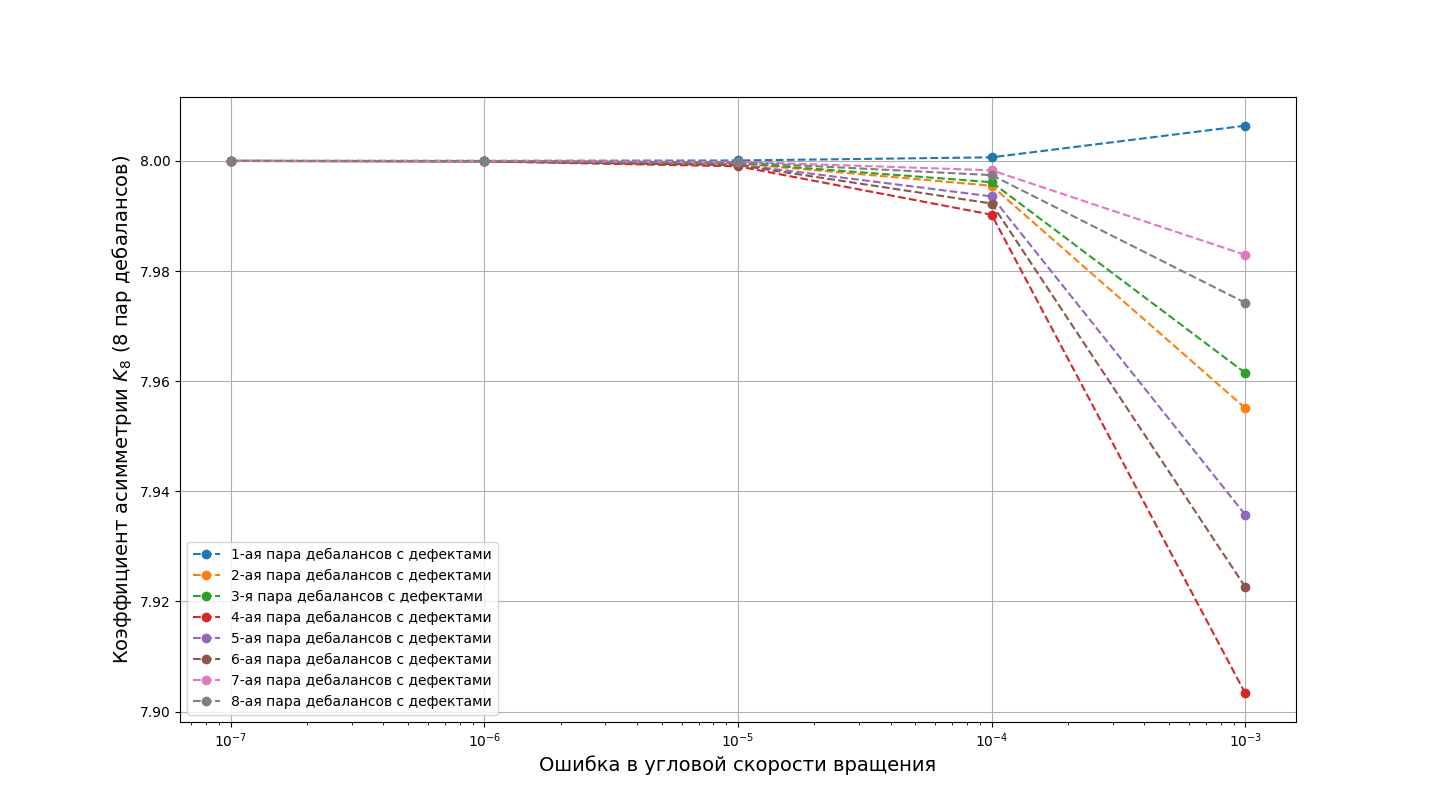
\includegraphics[width=1\linewidth]{pairs_with_defects_8}
    \caption{График изменения коэффициента ассиметрии для каждой пары дебалансов и погрешностей изготовления.
    Количество пар дебалансов -- 6 (график выше) и 8 (график ниже).}
    \label{fig:pairs_with_defects_even}
\end{figure}

\clearpage

\section*{Заключение}
\addcontentsline{toc}{section}{Заключение}

Целью этой работы является составление математической модели импульсного погружателя с дефектами одной пары дебалансов.
Определение, с использованием полученной модели, номера наиболее значимой пары дебалансов в процессе погружения.
Результатом этой работы будет служить программа, которая решает задачу поставленную выше.

В ходе данной работы была описана математичская модель импульсного погружателя с дефектами одной пары дебалансов. Была
написана программа, определяющая номер наиболее значимой пары дебалансов в процессе погружения. Было выяснено влияние на процесс погружения, оказываемое всеми парами дебалансами с дефектами и каждой из них в отдельности.

Также одним из результатов работы стал факт того, что в случае четного числа пар дебалансов с дефектами наблюдается
рост коэффициента асимметрии. Была поставлена задача по дальнейшему исследованию этого явления.

\clearpage

\addcontentsline{toc}{section}{Список литературы}

\nocite{*}

\printbibliography{}

\clearpage

\section*{Приложение}
\addcontentsline{toc}{section}{Приложение}

\subsection*{1. Расчёт коэффициента асимметрии с дефектами одной пары дебалансов}
\inputminted[linenos, fontsize=\footnotesize]{python}{app/acoeff.py}

\subsection*{2. Моделирование процесса погружения сваи}
\inputminted[linenos, fontsize=\footnotesize]{python}{app/main.py}

\subsection*{3. График движущей силы вибрационного погружателя и импульсного погружателя}
\inputminted[linenos, fontsize=\footnotesize]{python}{app/impuls.py}
